%In the drone
\newpage
\subsection{Acidity} \label{acidity}
Acidity is the quantitative capacity of a water or solution to neutralize an alkali. pH is a measure of the acidity or basicity of an aqueous solution. Solutions with a pH less than 7 are said to be acidic and solutions with a pH greater than 7 are basic or alkaline. \cite{phmerriam} Acidity can be interpreted in terms of specific substances only when the chemical composition of the sample is known. In this section, a closer look is taken at pH and how it affects the water quality. 

\subsubsection{Temperature}
The pH is inversely proportional to the temperature of the solution. When the temperature of a solution rises, the molecular vibrations in the solution rise resulting in the ionization and formation of H+ ions. More H+ ions lead to more acidic behavior. Generally, if we increase the temperature by 10°C, the pH of a solution or a substance will drop by 0.2.  \cite{temperatureph}

\subsubsection{Corrosion}
The pH is inversely proportional to the rate of corrosion. Corrosion occurs due to the formation of electrochemical cells. Low pH acid waters accelerate corrosion by providing a plentiful supply of hydrogen ions. The metal acts like an anode, with more negative potential with respect to the water which acts like a cathode. \cite{standardmethods}

\subsubsection{The carbon dioxide equilibrium system}
One of the most important chemical properties of water is that it can be both an acid and a base, because water ionizes into H+ and OH- ions.
The ionization is an equilibrium reaction.\\
The concentration of $H^+$ is usually denoted as the negative logarithm pH, while the concentration of $OH^-$ is denoted as the negative logarithm pOH.
For a neutral solution with a pH/pOH of 7.0 at 25 degrees celsius:
\[H^+ = OH^- = 0.0001 mmol/L\]
A lower pH than 7.0, meaning a higher concentration of H+ ions, indicates an acid solution. Water with a pH above 7 is a base. The pH of most raw water lies within the range 6.5–8.5 \cite{standardmethods}\\

The most important acid-base reaction in water is related to the dissociation of carbon dioxide. \cite{aes} When $CO_2$ becomes aqueous in water, a small portion of it becomes $H_2CO_3$, leaving $H^+$ ions:
\[CO_2 + H^2O <=> H^+ + HCO_3\]
$HCO_3^-$ can at it's turn release another $H^+$ ion:
\[HCO_3^- <=> CO_3^{2-} + H^+\]
The amount of carbon dioxide $CO_2$ in solution can determine the pH of the water. The most common source of acidity in water is dissolved $CO_2$, so the more $CO_2$ in the water, the lower the pH. As seen, dissolved $CO_2$ undergoes different stages over time. These stages have different pH levels associated with them:

\begin{figure}[h]
\centering
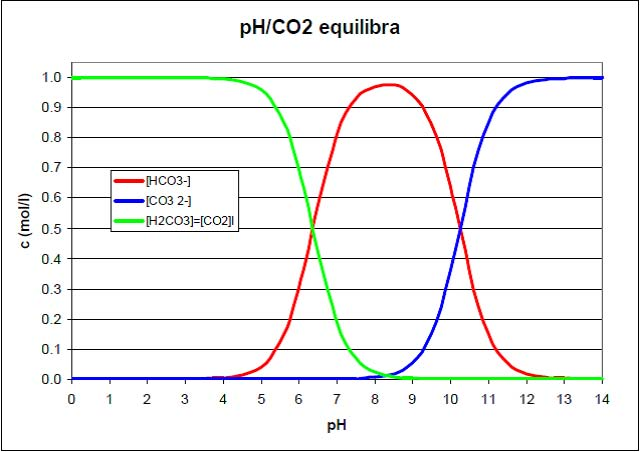
\includegraphics[scale=0.9]{water/21_equilibrium.jpg}
\caption{pH/$CO_2$ equilibrium \cite{aes}}
\end{figure}

\newpage
\subsubsection{Sensors}
In this section, a comparison between potential acidity (pH) sensors for the project is given. Certain features like price, accuracy, and form factor will be given.

To ensure accuracy, a pH probe needs to be calibrated first in two buffer solutions, pH 4.0 and pH 7.0. This has to be done every month. These buffer solutions usually cost around €15,- or can be found in most chemistry labs. As the pH is inversely proportional to the temperature of the solution, one should also use a temperature sensor to get meaningful data.

\paragraph{DFRobot Gravity V2}\mbox{€35.92} \cite{SEN0161V2}
\begin{table}[h!]
	\centering
	\adjustimage{height=4cm,valign=c}{water/22_gravityv2.jpg}\quad
	\begin{tabular}{| l | l |}
    \hline
    Interface & Analog \\
    Measurement Range & 0-14 pH \\
    Measurement Accuracy &  0.1pH \\
    Response time & Within 2min \\
    Supply Voltage & 3.3V-5V \\
    Software library included & yes \\
    Long term immersion & no \\
    Availability & 3-5 Working Days \\
    \hline
	\end{tabular}
\end{table}

\newpage
\paragraph{DFRobot Gravity V2 Pro}\mbox{€59,01} \cite{SEN0169V2}
\begin{table}[h!]
	\centering
	\adjustimage{height=4cm,valign=c}{water/23_gravityv2pro.jpg}\quad
	\begin{tabular}{| l | l |}
    \hline
    Interface & Analog \\
    Measurement Range & 0-14 pH \\
    Measurement Accuracy &  0.1pH \\
    Response time & Within 1min \\
    Supply Voltage & 3.3V-5V \\
    Software library included & yes \\
    Long term immersion & yes \\
    Availability & 3-5 Working Days \\
    \hline
	\end{tabular}
\end{table}


\paragraph{Generic PH0-14}\mbox{€15,83} \cite{PH0-14}
\begin{table}[h!]
	\centering
	\adjustimage{height=4cm,valign=c}{water/24_ph014.jpg}\quad
	\begin{tabular}{| l | l |}
    \hline
    Interface & Analog \\
    Measurement Range & 0-14 pH \\
    Measurement Accuracy &  0.25pH \\
    Response time & Within 1min \\
    Supply Voltage & 3.3V-5V \\
    Software library included & no \\
    Long term immersion & no \\
    Availability & 26 Days \\
    \hline
	\end{tabular}
\end{table}


